\documentclass[a4paper,12pt]{report}
\usepackage[utf8]{inputenc}
\usepackage[czech]{babel}
\usepackage{amsmath}
\usepackage{geometry}
\usepackage{xcolor}
\usepackage{graphicx}
\usepackage{fancyhdr}
\usepackage{soul}
\usepackage{array}
\usepackage{pgf}
\usepackage{enumitem}
\usepackage[normalem]{ulem}
\usepackage{hyperref}
\usepackage[figurename=Obr.,tablename=Tab.]{caption}
\usepackage{placeins}
\usepackage{amssymb}

\geometry{top=2.5cm, bottom=2.5cm, left=2.0cm, right=2.0cm}

% Variables, fill it here!
\newcommand{\sourceId}   {166}
\newcommand{\studentName}{Bc. Pavel Mikula}
\newcommand{\studentID}  {MIK0486}
\newcommand{\teacherName}{Ing. Michal Béreš, Ph.D.}

\renewcommand{\headrulewidth}{0pt}
\renewcommand{\footrulewidth}{0pt}

% Table and Image references
\newcommand{\tabref}[1]{Tab. \ref{#1}}
\newcommand{\figref}[1]{Obr. \ref{#1}}

% TODO command, to show spaces where to fill requested values more easily
\newcommand{\TODO}{\mbox{\textbf{\textcolor{red}{...} }}}

\pagestyle{fancy}
\fancyhead[L]{\colorbox{yellow}{\parbox{\dimexpr\textwidth-2\fboxsep\relax}{Jméno: \studentName}}}
\fancyhead[C]{\colorbox{yellow}{\parbox{\dimexpr\textwidth-2\fboxsep\relax}{}}}
\fancyhead[R]{\colorbox{yellow}{}{Číslo zadání: \sourceId}}

% Type of table columns that orients text to center
\newcolumntype{P}[1]{>{\centering\arraybackslash}p{#1}}

\begin{document}
\thispagestyle{empty}
\setcounter{page}{0}

% Title and header section
\begin{center}
    
\includegraphics[width=0.8\textwidth]{assets/logo.png} \\[4em]
    \vspace{4em}
    \textbf{PRAVDĚPODOBNOST A STATISTIKA} \\
    \vspace{1em}
    \textbf{Domácí úkoly 1S \textendash\ 3S} \\
    \textbf{\colorbox{yellow}{Zadání \sourceId}} \\
\end{center}

% Student information, values are implemented in variable section above
\vspace{2em}
\hspace{3em}
\begin{tabular}{ll}
    \textbf{Jméno studentky/studenta:}  & \hspace{6em} \studentName \\[0.5em]
    \textbf{Osobní číslo:}              & \hspace{6em} \studentID   \\[0.5em]
    \textbf{Jméno cvičící/cvičícího:}   & \hspace{6em} \teacherName \\
\end{tabular}

% Table with results
\vspace{10em}
\begin{center}
    \renewcommand{\arraystretch}{1.3}
    \begin{tabular}{|p{8em}|P{10em}|P{10em}|}
        \hline
                        & \textbf{Datum odevzdání}  & \textbf{Hodnocení}    \\ \hline
        Domácí úkol 1:  & 17.11.2024                & 6.0b                  \\ \hline
        Domácí úkol 2:  & 31.11.2024                & 7.0b                  \\ \hline
        Domácí úkol 3:  & 06.12.2024                &                       \\ \hline
        Celkem:         & ------------------------  &                       \\ \hline
    \end{tabular}
\end{center}

% Footer section
\vspace{5em}
\begin{center}
    \textbf{Ostrava, AR 2024/2025}
\end{center}

%\newpage
\section*{Popis datového souboru}
\label{sec:data-source-description}

V datovém souboru jsou zaznamenány výkonnostní skóre (FPS) čtyř populárních grafických karet:
Nvidia RTX 2080 Ti, Nvidia RTX 3070 Ti, AMD Radeon RX 6800 XT a AMD Radeon RX 7700 XT. Tyto karty
byly testovány ve hře "Cyberpunk 2077" ve dvou různých verzích: původní release a po aplikaci 1.5
patche. Vaším úkolem je analyzovat, jak patch 1.5 ovlivnil výkonnostní skóre těchto karet ve hře. Pro
každý unikátní testovaný systém (test) viz (id) byly testovány obě verze hry

\vspace{1em}
\noindent
V souboru ukol\_X.xlsx jsou pro každý test uvedeny následující údaje:

\begin{itemize}
  \item \textbf{id} ... identifikátor testovaného systému (každý systém je unikátní PC systém)
  \item \textbf{typ karty} ... Nvidia RTX 2080 Ti, Nvidia RTX 3070 Ti, AMD Radeon RX 6800 XT, AMD Radeon RX 7700 XT
  \item \textbf{testovaná verze} ... „release“ a „patched“
  \item \textbf{FPS} ... naměřené výkonnostní skóre (FPS) pro danou grafickou kartu s danou verzi hry.
\end{itemize}

\noindent
Obecné pokyny:

\begin{itemize}
    \item Domácí úkoly odevzdávejte vždy v termínu, který určil váš cvičící.
    \item Portfolio domácích úkolů budete odevzdávat postupně. Tj. nejdříve odevzdáte titulní stránku s úkolem 1, k okomentovanému úkolu 1 připojíte úkol 2 atd
    \item Domácí úkoly zpracujte dle obecně známých typografických pravidel. 
    \item Všechny tabulky i obrázky musí být opatřeny titulkem, který obsahuje i očíslování objektu.  
    \item Do domácích úkolů nevkládejte tabulky a obrázky, na něž se v doprovodném textu nebudete odkazovat.
    \item Bude-li to potřeba, citujte zdroje dle mezinárodně platné citační normy ČSN ISO 690.
\end{itemize}

\endinput

\newpage
\section*{Úkol 1}
\label{sec:task-1}

Pomocí nástrojů explorační analýzy zkoumejte nárůst výkonnostních skóre (FPS) po aplikaci 1.5 patche 
(tj. rozdíl výkonnostních skóre pro verzi „patched“ a verzi „release“) ve hře "Cyberpunk 2077" pro grafické karty 
\nvidiaCard\ a \amdCard\. Data vhodně graficky prezentujte (krabicový graf, histogram, q-q graf)
a doplňte následující tabulku a text.

\vspace{2em}
\noindent
Výsledky popisné statistiky lze vidět v \tabref{tab:characteristics-summary} a na  \figref{fig:box_plot}, \figref{fig:histogram} a \figref{fig:qq}.

% Fill your table values here :)
\newcommand{\rangeValues}       {70,        59,         69,         58}
\newcommand{\minValues}         {-4.8,      4.2,        5.1,        4.2}
\newcommand{\QfValues}          {5.425,     4.900,      5.500,      4.900}
\newcommand{\medianValues}      {5.700,     5.300,      5.700,      5.300}
\newcommand{\meanValues}        {5.600,     5.371,      5.750,      5.191}
\newcommand{\QtValues}          {6.100,     5.550,      6.100,      5.500}
\newcommand{\maxValues}         {6.6,       15.8,       6.6,        5.9}
\newcommand{\sdValues}          {1.335,     1.452,      0.439,      0.451}
\newcommand{\cvValues}          {23.8,      27.0,       7.6,        8.7}
\newcommand{\skewnessValues}    {-6.9,      6.4,        0.2,        -0.4}
\newcommand{\kurtosisValues}    {51.3,      43.8,       -1.0,       -0.7}
\newcommand{\lowerBoundValues}  {4.41,      3.92,       0,          0}
\newcommand{\upperBoundValues}  {7.11,      6.52,       0,          0}

% Additional values
\newcommand{\sigmaValues} {4.873, 6.628, 4.289, 6.093}

% Helper command to put everything in table.
\newcommand{\tableValue}[2]{%
    \pgfmathparse{{#1}[#2]}%
    \edef\tempResult{\pgfmathresult}%
    \ifnum\pdfstrcmp{\tempResult}{inf}=0 %
        $\infty$%
    \else%
        \mbox{\tempResult}%
    \fi%
}

% Fuckin graphic card names
\newcommand{\nvidiaCard}{Nvidia RTX 3070 Ti}
\newcommand{\amdCard} {AMD Radeon RX 7700 XT}

\begin{table}[h!]
    \caption{Nárůst výkonnostních skóre (FPS) po aplikaci 1.5 patche ve hře "Cyberpunk 2077" pro grafické karty \nvidiaCard\ a \amdCard\ (souhrnné statistiky)}
    \label{tab:characteristics-summary}
    \vspace{0.5em}
    \renewcommand{\arraystretch}{1.3}
    \resizebox{\textwidth}{!}{%
        \begin{tabular}{|p{3.5cm}|P{3cm}|P{3cm}|P{3cm}|P{3cm}|}
            \hline
                                  & \multicolumn{2}{P{6cm}|}{\textbf{Původní data}}                   & \multicolumn{2}{P{6cm}|}{\textbf{Data po odstranění odlehlých pozorování}} \\ \hline
                                  & \centering \textbf{\nvidiaCard} & \textbf{\amdCard}               & \centering \textbf{\nvidiaCard} & \textbf{\amdCard}                        \\ \hline
            rozsah souboru        & \tableValue{\rangeValues}{0}    & \tableValue{\rangeValues}{1}    & \tableValue{\rangeValues}{2}    & \tableValue{\rangeValues}{3}             \\ \hline
            minimum               & \tableValue{\minValues}{0}      & \tableValue{\minValues}{1}      & \tableValue{\minValues}{2}      & \tableValue{\minValues}{3}               \\ \hline
            dolní kvartil         & \tableValue{\QfValues}{0}       & \tableValue{\QfValues}{1}       & \tableValue{\QfValues}{2}       & \tableValue{\QfValues}{3}                \\ \hline
            medián                & \tableValue{\medianValues}{0}   & \tableValue{\medianValues}{1}   & \tableValue{\medianValues}{2}   & \tableValue{\medianValues}{3}            \\ \hline
            průměr                & \tableValue{\meanValues}{0}     & \tableValue{\meanValues}{1}     & \tableValue{\meanValues}{2}     & \tableValue{\meanValues}{3}              \\ \hline
            horní kvartil         & \tableValue{\QtValues}{0}       & \tableValue{\QtValues}{1}       & \tableValue{\QtValues}{2}       & \tableValue{\QtValues}{3}                \\ \hline
            maximum               & \tableValue{\maxValues}{0}      & \tableValue{\maxValues}{1}      & \tableValue{\maxValues}{2}      & \tableValue{\maxValues}{3}               \\ \hline
            směrodat. odchylka    & \tableValue{\sdValues}{0}       & \tableValue{\sdValues}{1}       & \tableValue{\sdValues}{2}       & \tableValue{\sdValues}{3}                \\ \hline
            variační koefi. (\%)  & \tableValue{\cvValues}{0}       & \tableValue{\cvValues}{1}       & \tableValue{\cvValues}{2}       & \tableValue{\cvValues}{3}                \\ \hline
            šikmost               & \tableValue{\skewnessValues}{0} & \tableValue{\skewnessValues}{1} & \tableValue{\skewnessValues}{2} & \tableValue{\skewnessValues}{3}          \\ \hline
            špičatost             & \tableValue{\kurtosisValues}{0} & \tableValue{\kurtosisValues}{1} & \tableValue{\kurtosisValues}{2} & \tableValue{\kurtosisValues}{3}          \\ \hline
            \multicolumn{5}{|p{16cm}|}{\textbf{Identifikace odlehlých pozorování (vnitřní hradby)}} \\ \hline
            dolní mez   & \tableValue{\lowerBoundValues}{0} & \tableValue{\lowerBoundValues}{1} & \multicolumn{2}{P{6cm}|}{------------} \\ \hline
            horní mez   & \tableValue{\upperBoundValues}{0} & \tableValue{\upperBoundValues}{1} & \multicolumn{2}{P{6cm}|}{------------} \\ \hline
        \end{tabular}%
    }
\end{table}

\newpage
\noindent
\textbf{Grafická prezentace (krabicový graf, histogram, q-q graf)}

\begin{figure}[h!]
    \centering
    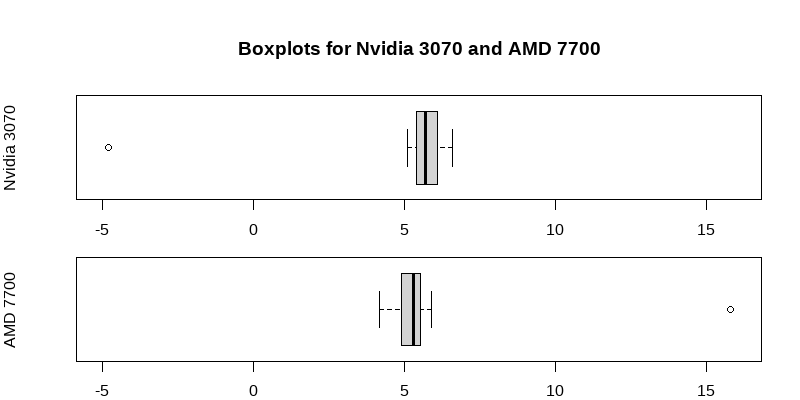
\includegraphics[width=0.75\textwidth]{assets/box_plot}
    \caption{Krabicový graf znázorňující rozložení nárůstu FPS po aplikaci 1.5 patche ve hře "Cyberpunk 2077" pro grafické karty \nvidiaCard\ a \amdCard}
    \label{fig:box_plot}
\end{figure}

\begin{figure}[h!]
    \centering
    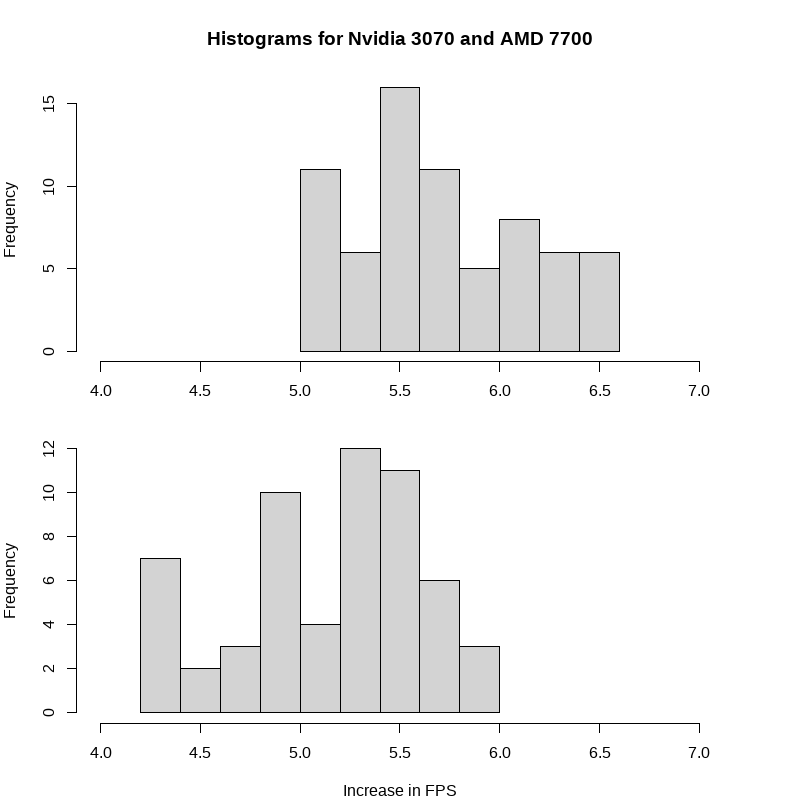
\includegraphics[width=0.75\textwidth]{assets/histogram}
    \caption{Histogram znázorňující rozložení nárůstu FPS po aplikaci 1.5 patche ve hře "Cyberpunk 2077" pro grafické karty \nvidiaCard\ a \amdCard}
    \label{fig:histogram}
\end{figure}

\begin{figure}[h!]
    \centering
    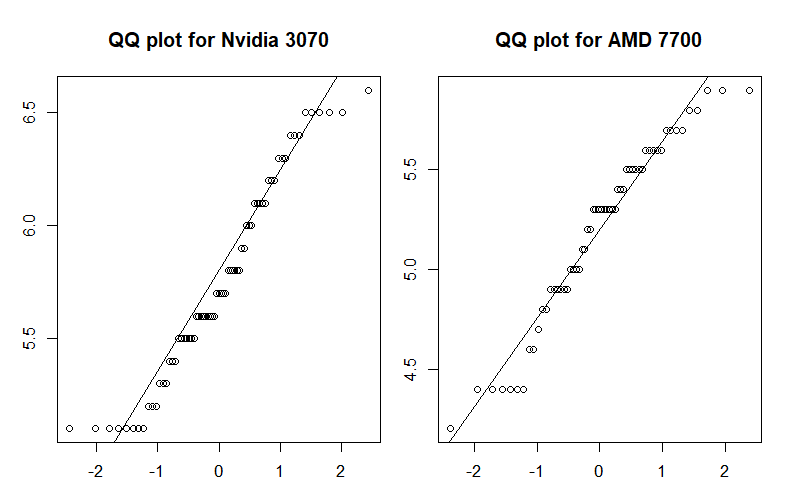
\includegraphics[width=0.85\textwidth]{assets/qq}
    \caption{Q-Q graf znázorňující nárůst FPS po aplikaci 1.5 patche ve hře "Cyberpunk 2077" pro grafické karty \nvidiaCard\ a \amdCard}
    \label{fig:qq}
\end{figure}

\newpage
\subsubsection*{Analýza nárůstu výkonnostních skóre (FPS) po aplikaci 1.5 patche ve hře "Cyberpunk 2077" pro grafickou kartu \nvidiaCard}

Během testu byl zjišťován nárůst FPS pro grafickou kartu \nvidiaCard\ ve hře "Cyberpunk 2077" mezi původním release a verzí s 1.5 patchem
pro \tableValue{\rangeValues}{0} testovacích systémů. Zjištěný nárůst FPS se pohyboval v rozmezí \tableValue{\minValues}{0} FPS
až \tableValue{\maxValues}{0} FPS. Nárůst FPS v testu č. 20 byl na základě metody vnitřních hradeb identifikován jako odlehlé pozorování
a nebude zahrnut do dalšího zpracování. Možné příčiny vzniku odlehlých pozorování jsou: Chyba při testování vzniklá náhlým výkyvem výkonu počítače
nebo chyba hardwaru výpočetní stanice. Dále uvedené výsledky tedy pocházejí z analýzy nárůstů FPS zjištěných u \tableValue{\rangeValues}{2}
testovacích systémů. Průměrný nárůst FPS byl \tableValue{\meanValues}{2} FPS, směrodatná odchylka pak \tableValue{\sdValues}{2} FPS\@.
U poloviny testovacích cyklů nárůst FPS nepřekročil \tableValue{\medianValues}{2} FPS. V polovině případů se nárůst FPS pohyboval v
rozmezí \tableValue{\QfValues}{2} FPS až \tableValue{\QtValues}{2} FPS. Vzhledem k povaze měřené veličiny není variační koeficient vhodnou mírou
pro posouzení variability souboru.

\vspace{1em}
\noindent
Výsledky pro grafickou kartu AMD Radeon RX 7700 XT lze komentovat obdobně.
Nárůst FPS se pohyboval v rozmezí \tableValue{\minValues}{1} až \tableValue{\maxValues}{1} FPS, s průměrným nárůstem \tableValue{\meanValues}{3} FPS a
směrodatnou odchylkou \tableValue{\sdValues}{3} FPS.\@
Za pomocí metody vnitřních hradeb bylo identifikováno odlehlé pozorování v testu č.\ 24, které bylo z analýzy vyloučeno.
Medián nárůstu činil \tableValue{\medianValues}{3} FPS, přičemž polovina výsledků spadala do intervalu \tableValue{\QfValues}{3} až \tableValue{\QtValues}{3} FPS.\@
Opět i zde není variační koeficient vhodným měřítkem variability souboru.

\subsubsection*{Ověření normality nárůstu výkonnostních skóre (FPS) po aplikaci 1.5 patche ve hře "Cyberpunk 2077" pro grafickou kartu \nvidiaCard}

Na základě grafického zobrazení (viz \figref{fig:qq}) u grafické karty \nvidiaCard\ a výběrové šikmosti a špičatosti (viz \tabref{tab:characteristics-summary},
výběrová šikmost a špičatost leží v intervalu (-2, 2)) lze předpokládat, že pozorovaný nárůst FPS má normální rozdělení. Dle pravidla 3$\sigma$ lze tedy očekávat,
že přibližně u 95 \% naměřených nárůstů ve výkonu bude \tableValue{\sigmaValues}{0} FPS až \tableValue{\sigmaValues}{1} FPS\@.

\subsubsection*{Ověření normality nárůstu výkonnostních skóre (FPS) po aplikaci 1.5 patche ve hře "Cyberpunk 2077" pro grafickou kartu \amdCard}

Na základě grafického zobrazení (viz \figref{fig:qq}) u grafické karty \amdCard\ a výběrové šikmosti a špičatosti (viz \tabref{tab:characteristics-summary},
výběrová šikmost a špičatost leží v intervalu (-2, 2)) lze předpokládat, že pozorovaný nárůst FPS má normální rozdělení. Dle pravidla 3$\sigma$ lze tedy očekávat,
že přibližně u 95 \% naměřených nárůstů ve výkonu bude \tableValue{\sigmaValues}{2} FPS až \tableValue{\sigmaValues}{3} FPS\@.

\endinput

\newpage
\section*{Úkol 2}
\label{sec:task-2}

Porovnejte nárůsty ve výkonnostních skórech (FPS) pro verzi hry "Cyberpunk 2077" po aplikaci 1.5 patche (dále jen \textbf{„nárůst FPS“}) 
pro vybrané grafické karty. Nezapomeňte, že použité metody mohou vyžadovat splnění určitých předpokladů. Pokud tomu tak bude, okomentujte 
splnění/nesplnění těchto předpokladů jak na základě explorační analýzy (např. s odkazem na histogram apod.), tak exaktně pomocí metod statistické indukce.

\newcommand{\lowerThanZero}{$<$$<$ 0.001}

\newcommand{\shapireWilk}{0.006, 0.019}
\newcommand{\symmetryTest}{0.218, 0.016}
\newcommand{\ttValues}{5.600, "inf", 5.100, "inf"}
\newcommand{\rtxInterval}{(\tableValue{\ttValues}{0}, \tableValue{\ttValues}{1}) }
\newcommand{\amdInterval}{(\tableValue{\ttValues}{2}, \tableValue{\ttValues}{3}) }

\newcommand{\pointGuess}{0.400}
\newcommand{\wilcoxLeftSidedInterval}{$(0.399, \infty)$}

\begin{enumerate}[label=\alph*)]
    \item Graficky prezentujte srovnání nárůstu FPS pro grafické karty \nvidiaCardTri\ a \amdCardSedm\ (vícenásobný krabicový graf, histogramy, q-q grafy).
    Srovnání okomentujte (včetně informace o případné manipulaci s datovým souborem).

    \vspace{1em}
    \begin{minipage}{0.94\textwidth}
        Pro srovnání nárůstu FPS pro jednotlivé grafické karty je možné využít krabicový graf na \figref{fig:box_plot}, histogramy na \figref{fig:histogram} a q-q grafy na \figref{fig:qq}.
        V těchto grafech již nejsou zobrazeny odlehlé hodnoty, které byly identifikovány v úkolu 1.
    \end{minipage}

    \newpage
    \item Na hladině významnosti 5 \% rozhodněte, zda jsou střední hodnoty nárůstů FPS (popř.\ mediány nárustů FPS) pro grafické karty \nvidiaCardTri\ a
    \amdCardSedm\ statisticky významné.\ K řešení využijte bodové a intervalové odhady i čistý test významnosti.\ Výsledky okomentujte.

    \vspace{1em}
    \begin{minipage}{0.94\textwidth}
        Na základě prezentovaných Q-Q grafů (viz \figref{fig:qq}) lze usuzovat, že nárůst FPS u obou grafických karet odpovídá normálnímu rozdělení.
        Toto tvrzení podporují i hodnoty výběrové šikmosti a špičatosti, které spadají do intervalu (-2, 2) (viz \tabref{tab:characteristics-summary}). \\

        Dle Shapirova-Wilkova testu (viz \tabref{tab:normality-test}) nelze na hladině významnosti 0.05 nárůst FPS obou typů grafických karet považovat za normálně rozdělený.
        Z toho důvodu je nutné použít neparametrické testy pro ověření významnosti mediánu nárůstu FPS (viz \tabref{tab:deterministic-normality-test}).

        \captionof{table}{Ověření normality nárůstu FPS dle grafických karet}
        \label{tab:normality-test}
        \renewcommand{\arraystretch}{1.3}
        \resizebox{\textwidth}{!}{%
            \begin{tabular}{|p{5cm}|P{3.5cm}|P{3.5cm}|P{8cm}|}
                \hline
                            & \textbf{šikmost}                & \textbf{špičatost}              & \textbf{Shapirův-Wilkův test (p-hodnota)} \\ \hline
                \nvidiaCardTri & \tableValue{\skewnessValues}{2} & \tableValue{\kurtosisValues}{2} & \tableValue{\shapireWilk}{0}              \\ \hline
                \amdCardSedm    & \tableValue{\skewnessValues}{3} & \tableValue{\kurtosisValues}{3} & \tableValue{\shapireWilk}{1}              \\ \hline
            \end{tabular}%
        }
        \vspace{1em}

        % TODO: Barče, použít u obou Wilcoxon??
        Na základě testu symetrie (viz \tabref{tab:deterministic-normality-test}) bylo u grafické karty \nvidiaCardTri\ nebylo zamítnuto symetrické rozdělení, zatímco u grafické karty \amdCardSedm\ bylo.\@
        Vzhledem k tomu, že výsledky scheme srovnávat tak budeme dále předpokládat, že nárůst FPS u obou grafických karet není symetrický.
        Po provedení SIGN testu bylo zjištěno, že medián nárůstu FPS je pro obě grafické karty významně vyšší než 0.
        Lze tedy konstatovat, že medián nárůstu FPS je pro obě grafické karty statisticky významný.

        \captionof{table}{Podrobné ověření normality nárůstu FPS dle grafických karet}
        \label{tab:deterministic-normality-test}
        \vspace{0.5em}
        \renewcommand{\arraystretch}{1.3}
        \resizebox{\textwidth}{!}{%
            \begin{tabular}{|p{5cm}|P{5cm}|P{10cm}|}
                \hline
                            & \textbf{Test symetrie}        & \textbf{SIGN test} \\ \hline
                \nvidiaCardTri & \tableValue{\symmetryTest}{0} & \lowerThanZero     \\ \hline
                \amdCardSedm    & \tableValue{\symmetryTest}{1} & \lowerThanZero     \\ \hline
            \end{tabular}%
        }
        \vspace{1em}

        Vzhledem k tomu, že očekáváme kladné hodnoty nárůstu FPS (výkonnostní skóre se zvyšuje), volíme levostranné intervalové odhady a levostranné testy.
        U grafické karty \nvidiaCardTri\ lze očekávat, že průměrný nárůst FPS bude přibližně \tableValue{\meanValues}{2}.\@
        95\% levostranný intervalový odhad průměrného nárůstu FPS pro tuto kartu je \rtxInterval FPS.\@
        Intervalový odhad i p-hodnota levostranného t-testu ukazují, že průměrný nárůst FPS je statisticky významně větší než nula.
        Jinými slovy, na hladině významnosti 0,05 lze nárůst FPS pro grafickou kartu \nvidiaCardTri\ považovat za statisticky významný. \\

        U grafické karty \amdCardSedm\ lze odhady interpretovat obdobně.
        Nárůst FPS pro tuto kartu je přibližně \tableValue{\meanValues}{3}.\@ a 95\% levostranný intervalový odhad průměrného nárůstu FPS je \amdInterval FPS.\@

        \captionof{table}{Bodové a intervalové odhady střední hodnoty nárůstu FPS dle grafických karet}
        \label{tab:interval-estimation}
        \vspace{0.5em}
        \renewcommand{\arraystretch}{1.3}
        \resizebox{\textwidth}{!}{%
            \begin{tabular}{|p{5cm}|P{4cm}|P{7cm}|P{4cm}|}
                \hline
                            & \textbf{bodový odhad (FPS)} & \textbf{95\% levostranný intervalový odhad (FPS)} & \textbf{Levostranný t-test (p-hodnota)} \\ \hline
                \nvidiaCardTri & \tableValue{\meanValues}{2} & \rtxInterval                                      & \lowerThanZero                          \\ \hline
                \amdCardSedm    & \tableValue{\meanValues}{3} & \amdInterval                                      & \lowerThanZero                          \\ \hline
            \end{tabular}%
        }
    \end{minipage}

    \newpage
    \item Pro grafické karty \nvidiaCardTri\ a \amdCardSedm\ rozhodněte (na hladině významnosti 5 \%), zda se jejich střední hodnoty (popř.\ mediány)
    nárůstu FPS po aplikaci 1.5 patche statisticky významně liší.
    K řešení využijte bodový a intervalový odhad i čistý test významnosti.
    Výsledky okomentujte.

    \vspace{1em}
    \begin{minipage}{0.94\textwidth}
        Vzhledem k zamítnutí předpokladu normality nárůstu FPS (viz \tabref{tab:normality-test}) budeme i nadále pokračovat v aplikaci neparametrických metod. \\

        Tvar rozdělení nárůstu FPS u obou grafických karet je srovnatelný (viz \figref{fig:histogram}).
        Pro odhad a test významnosti rozdílu mediánů nárůstu FPS využijeme metody založené na Mannově-Whitneyho statistice.

        \captionof{table}{Srovnání mediánů nárustu FPS grafické karty \nvidiaCardTri\ a \amdCardSedm)}
        \label{tab:median-comparison}
        \vspace{0.5em}
        \renewcommand{\arraystretch}{1.3}
        \resizebox{\textwidth}{!}{%
            \begin{tabular}{p{12cm}P{3cm}}
                \hline
                \textbf{Bodový odhad $x^{Nvidia}_{0.5} - x^{AMD}_{0.5}$ (mAh)}                         & \pointGuess              \\
                \textbf{95\% levostranný intervalový odhad $x^{Nvidia}_{0.5} - x^{AMD}_{0.5}$ (mAh)}   & \wilcoxLeftSidedInterval \\
                \textbf{Mannův-Whitneyho levostranný test (p-hodnota)}                                 & \lowerThanZero           \\
                \hline
            \end{tabular}%
        }
        \vspace{1em}

        U grafické karty \nvidiaCardTri\ lze očekávat, že medián nárůstu FPS bude přibližně o \pointGuess\ větší než u grafické karty \amdCardSedm.\@
        Odpovídající 95\% levostranný intervalový odhad rozdílu mediánů je \wilcoxLeftSidedInterval.\@
        Mannův-Whitneyho levostranný test ukazuje, že nárůst FPS u grafické karty \nvidiaCardTri\ je na hladině významnosti 5\% statisticky významně
        vyšší než u grafické karty \amdCardSedm.\@
    \end{minipage}
\end{enumerate}

\endinput

\newpage
\section*{Úkol 3}
\label{sec:task-3}

Na hladině významnosti 5 \% rozhodněte, zda střední hodnoty (popř\. mediány) nárůstů FPS po aplikaci 1.5 patche statisticky významně závisí na typu grafické karty.
Posouzení proveďte nejprve na základě explorační analýzy a následně pomocí vhodného statistického testu, včetně ověření potřebných předpokladů.
V případě, že se nárůst FPS pro různé grafické karty statisticky významně liší, určete pořadí karet dle středního nárůstu FPS (popř\. mediánu nárůstu FPS).
\textbf{Poznámka:} \textit{Srovnání proveďte pro všechny čtyři typy grafických karet.}

\renewcommand{\skewnessValues}{-0.2, 0.2, 0.2, -0.4}
\renewcommand{\kurtosisValues}{-1.1, -1.0, -1.1, -0.7}
\renewcommand{\shapireWilk}   {0.012, 0.006, 0.005, 0.019}
\renewcommand{\symmetryTest}  {0.087, 0.218, 0.043, 0.016}

\renewcommand{\meanValues}{5.200, 5.700, 4.750, 5.300}
\renewcommand{\ttRtxValues} {4.950, 5.250, 5.600, 5.850}
\renewcommand{\ttAmdValues} {4.700, 4.900, 5.100, 5.345}
\renewcommand{\rtxDvaInterval} {(\tableValue{\ttRtxValues}{0}, \tableValue{\ttRtxValues}{1}) }
\renewcommand{\rtxTriInterval} {(\tableValue{\ttRtxValues}{2}, \tableValue{\ttRtxValues}{3}) }
\renewcommand{\amdSestInterval} {(\tableValue{\ttAmdValues}{0}, \tableValue{\ttAmdValues}{1}) }
\renewcommand{\amdSedmInterval} {(\tableValue{\ttAmdValues}{2}, \tableValue{\ttAmdValues}{3}) }

\begin{enumerate}[label=\alph*)]
    \item Daný problém vhodným způsobem graficky prezentujte (vícenásobný krabicový graf, histogramy, q-q grafy). 
    Srovnání okomentujte (včetně informace o případné manipulaci s datovým souborem).

    \newline{
        \begin{figure}[h!]
            \centering
            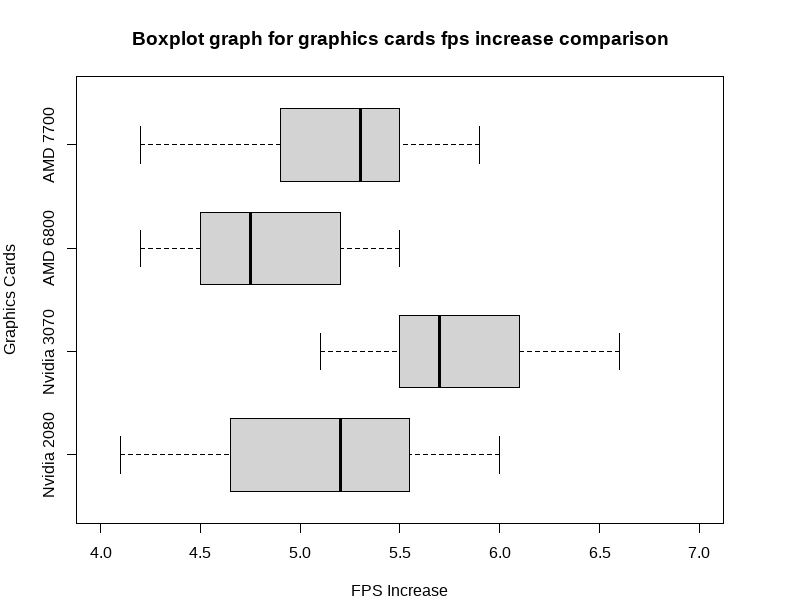
\includegraphics[width=0.75\textwidth]{assets/box_plot_all}
            \caption{Krabicový graf srovnávající nárůst FPS pro všechny čtyři grafické karty}
            \label{fig:box_plot_all}
        \end{figure}

        Pro další analýzu již použijeme data upravená o odlehlá pozorování. Dle \figref{fig:box_plot_all}, \figref{fig:histogram_all} a \figref{fig:qq_all} lze usuzovat, že nárůst FPS u grafické karty \nvidiaCardTri\ je výrazně vyšší než u ostatních grafických karet.

        \begin{figure}[h!]
            \centering
            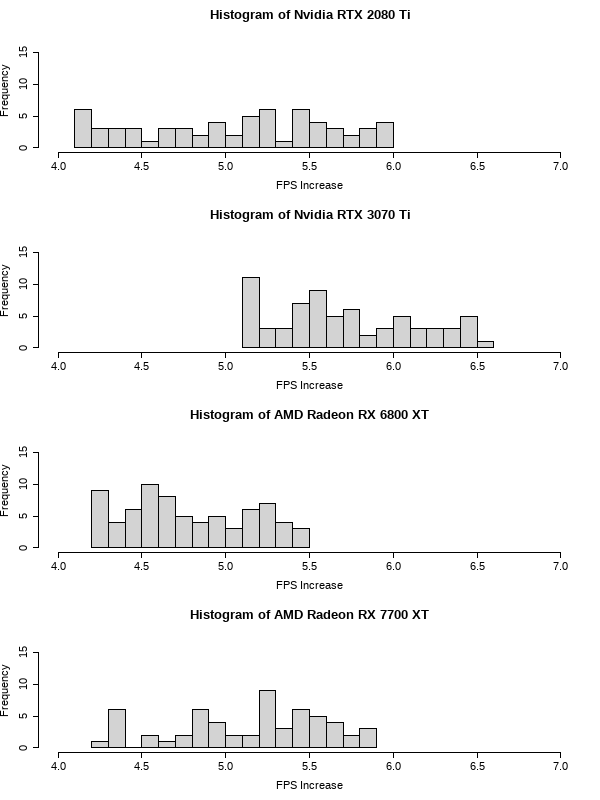
\includegraphics[width=0.75\textwidth]{assets/histograms_all}
            \caption{Histogramy srovnávající nárůst FPS pro všechny čtyři grafické karty}
            \label{fig:histogram_all}
        \end{figure}

        \begin{figure}[h!]
            \centering
            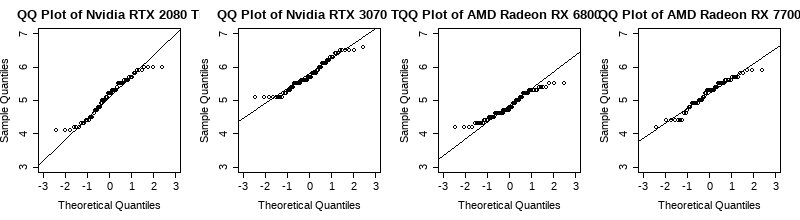
\includegraphics[width=1.0\textwidth]{assets/qq_all}
            \caption{Q-Q grafy srovnávající nárůst FPS pro všechny čtyři grafické karty}
            \label{fig:qq_all}
        \end{figure}
    }
    
    \newpage
    \item Ověřte normalitu a symetrii nárůstů FPS u všech čtyř grafických karet (empiricky i exaktně).

    \vspace{1em}
    \begin{minipage}{0.94\textwidth}
        Podle grafu Q-Q (viz \figref{fig:qq_all}), je viditelné, že nárůst FPS pro všechny grafické karty není v souladu s normálním rozdělením.
        Tomu ale neodpovídají hodnoty šikmosti a špičatosti, které se nacházejí v intervalu (-2, 2) (viz \tabref{tab:normality-test-all}).

        \vspace{1em}
        \captionof{table}{Ověření normality nárůstu FPS dle grafických karet}
        \label{tab:normality-test-all}
        \renewcommand{\arraystretch}{1.3}
        \resizebox{\textwidth}{!}{%
            \begin{tabular}{|p{5cm}|P{3.5cm}|P{3.5cm}|P{4cm}|P{4cm}|}
                \hline
                               & \textbf{šikmost}                & \textbf{špičatost}              & \textbf{Shapirův-Wilkův test (p-hodnota)} & \textbf{Test symetrie}        \\ \hline
                \nvidiaCardDva & \tableValue{\skewnessValues}{0} & \tableValue{\kurtosisValues}{0} & \tableValue{\shapireWilk}{0}              & \tableValue{\symmetryTest}{0} \\ \hline
                \nvidiaCardTri & \tableValue{\skewnessValues}{1} & \tableValue{\kurtosisValues}{1} & \tableValue{\shapireWilk}{1}              & \tableValue{\symmetryTest}{1} \\ \hline
                \amdCardSedm   & \tableValue{\skewnessValues}{2} & \tableValue{\kurtosisValues}{2} & \tableValue{\shapireWilk}{2}              & \tableValue{\symmetryTest}{2} \\ \hline
                \amdCardSest   & \tableValue{\skewnessValues}{3} & \tableValue{\kurtosisValues}{3} & \tableValue{\shapireWilk}{3}              & \tableValue{\symmetryTest}{3} \\ \hline
            \end{tabular}%
        }
        \vspace{1em}

        Dle Shapirova-Wilkova testu (viz \tabref{tab:normality-test-all}) nelze na hladině významnosti 0.05 nárust FPS u grafických karet považovat za normálně rozdělený.
        Z tohoto důvodu je nutné provést neparametrické testy. \\

        Po provedení testu symetrie, bylo zjištěno, že u grafických karet \nvidiaCardDva, \amdCardSedm a \amdCardSedm\ bylo zamítnuto symetrické rozdělení.
        A u grafické karty \nvidiaCardTri\ nebylo zamítnuto symetrické rozdělení. \\

        Proto v následující analýze budeme předpokládat, že nárůst FPS u všech grafických karet není symetrický.
    \end{minipage}

    \newpage
    \item Ověřte homoskedasticitu (shodu rozptylů) nárůstů FPS mezi jednotlivými kartami (empiricky i exaktně)

    \vspace{1em}
    \begin{minipage}{0.94\textwidth}
        Dle \figref{fig:box_plot_all} a výpočtu poměru největšího a nejmenšího rozptylu nárůstu FPS $(\frac{S^2_{max}}{S^2_{min}} \cong 2.3)$ se zdá, že srovnávané rozptyly nelze považovat za srovnatelné. \\

        Na základě Leveneho testu s výslednou p-hodnotou $0.006$ zamítáme předpoklad o shodě rozptylů nárůstu FPS mezi grafickými kartami.
    \end{minipage}
    
    \newpage
    \item Určete bodové a 95\% intervalové odhady střední hodnoty (popř\. mediánu) nárůstů FPS pro všechny srovnávané karty.
    Volbu charakteristik proveďte tak, aby byly v souladu se statistickým testem, který plánujete provést v bodě e). 
    (Nezapomeňte na ověření předpokladů pro použití příslušných intervalových odhadů.)

    \vspace{1em}
    \begin{minipage}{0.94\textwidth}
        Vzhledem k zamítnutí předpokladu o normalitě rozdělení nárůstů FPS mezi grafickými kartami použijeme Kruskalův-Wallisův test, který ověřuje shodu mediánů.
        Z tohoto důvodu využijeme mediány rovněž v rámci odhadu měr polohy.
        Pro určení intervalového odhadu byla použita Wilcoxonova statistika (viz \tabref{tab:interval-estimation-all}). \\

        Přestože její předpoklady (symetrie rozdělení) nejsou splněny, jedná se však o nejrobustnější test, který máme k dispozici.
        Jeho použití je tedy zvoleno s vědomím, že výsledky mohou být zkreslené a jejich interpretace by měla být prováděna obezřetně.

        \vspace{1em}
        \captionof{table}{Bodové a intervalové odhady mediánu nárůstů FPS dle grafických karet}
        \label{tab:interval-estimation-all}
        \vspace{0.5em}
        \renewcommand{\arraystretch}{1.3}
        \resizebox{\textwidth}{!}{%
            \begin{tabular}{|p{5cm}|P{6cm}|P{9cm}|}
                \hline
                                & \textbf{bodový odhad (FPS)} & \textbf{95\% levostranný intervalový odhad (FPS)} \\ \hline
                \nvidiaCardDva  & \tableValue{\meanValues}{0} & \rtxDvaInterval                                   \\ \hline
                \nvidiaCardTri  & \tableValue{\meanValues}{1} & \rtxTriInterval                                   \\ \hline
                \amdCardSest    & \tableValue{\meanValues}{2} & \amdSestInterval                                  \\ \hline
                \amdCardSedm    & \tableValue{\meanValues}{3} & \amdSedmInterval                                  \\ \hline
            \end{tabular}%
        }
        \vspace{1em}

        U poloviny testovacích cyklů nárůst FPS nepřekročil \tableValue{\meanValues}{0} FPS pro grafickou kartu \nvidiaCardDva.\@
        95\% intervalový odhad mediánu nárůstu FPS pro tuto grafickou kartu je \rtxDvaInterval\.\@ \\

        U poloviny testovacích cyklů nárůst FPS nepřekročil \tableValue{\meanValues}{1} FPS pro grafickou kartu \nvidiaCardTri.\@
        95\% intervalový odhad mediánu nárůstu FPS pro tuto grafickou kartu je \rtxTriInterval\.\@ \\

        U poloviny testovacích cyklů nárůst FPS nepřekročil \tableValue{\meanValues}{2} FPS pro grafickou kartu \amdCardSest.\@
        95\% intervalový odhad mediánu nárůstu FPS pro tuto grafickou kartu je \amdSestInterval\.\@ \\

        U poloviny testovacích cyklů nárůst FPS nepřekročil \tableValue{\meanValues}{3} FPS pro grafickou kartu \amdCardSedm.\@
        95\% intervalový odhad mediánu nárůstu FPS pro tuto grafickou kartu je \amdSedmInterval\.\@ \\

        Na grafické kartě \amdCardSest\ můžeme pozorovat nejnižší medián nárůstu FPS, který se oproti \nvidiaCardDva\ a \amdCardSedm\ liší o cca 0.450 FPS.\@
        Pro grafickou kartu \nvidiaCardTri\ je medián nárůstu FPS nejvyšší, a to o cca 0.400 FPS oproti oproti kartám \nvidiaCardDva\ a \amdCardSedm\!.
        Ty se od sebe liší zhruba o 0.100 FPS.\@
    \end{minipage}

    \newpage
    \item Čistým testem významnosti ověřte, zda je pozorovaný rozdíl středních hodnot (popř\. mediánů) nárůstů FPS statisticky
    významný na hladině významnosti 5\%.\@
    Pokud ano, zjistěte, zda lze některé skupiny karet označit (z hlediska nárůstů FPS) za homogenní, tj\. určete pořadí karet dle středních hodnot (popř\. mediánů) nárůstů FPS.\@
    (Nezapomeňte na ověření předpokladů pro použití zvoleného testu.) \\

    \begin{minipage}{0.94\textwidth}
        Na hladině významnosti 0.05 zamítáme hypotézu o shodě mediánů nárůstu FPS mezi grafickými kartami (Kruskalův-Wallisův test, p-hodnota $\ll 0.001$).
        Tzn.\ mediány nárůstu FPS se mezi grafickými kartami statisticky významně liší. \\

        Test byl proveden i přes to, že předpoklady (symetrie rozdělení) nejsou splněny, jedná se však o nejrobustnější test, který máme k dispozici.
        Jeho použití je tedy zvoleno s vědomím, že výsledky mohou být zkreslené a jejich interpretace by měla být prováděna obezřetně. \\

        Pro určení, které skupiny karet lze označit za homogenní, jsme použili Dunnův test s Bonferroniho korekcí (viz. \tabref{tab:post-hoc-test}).

        \vspace{1em}
        \captionof{table}{Efekty nárůstu FPS dle grafických karet}
        \label{tab:post-hoc-test}
        \vspace{0.5em}
        \renewcommand{\arraystretch}{1.3}
        \resizebox{\textwidth}{!}{%
            \begin{tabular}{|p{5cm}|P{15cm}|}
                \hline
                               & \textbf{Efekt} \\ \hline
                \nvidiaCardTri & $0.400$        \\ \hline
                \amdCardSedm   & $0$            \\ \hline
                \nvidiaCardDva & $-0.100$       \\ \hline
                \amdCardSest   & $-0.550$       \\ \hline
            \end{tabular}%
        }

        \vspace{1em}
        \captionof{table}{Adjustované p-hodnoty post-hoc analýzy}
        \label{tab:letter-test}
        \vspace{0.5em}
        \renewcommand{\arraystretch}{1.3}
        \resizebox{\textwidth}{!}{%
            \begin{tabular}{|p{5cm}|P{4cm}|P{4cm}|P{4cm}|P{4cm}|}
                \hline
                               & \nvidiaCardTri & \amdCardSedm   & \nvidiaCardDva & \amdCardSest   \\ \hline
                \nvidiaCardTri & -              & \lowerThanZero & \lowerThanZero & \lowerThanZero \\ \hline
                \amdCardSedm   & \lowerThanZero & -              & 1.000          & \lowerThanZero \\ \hline
                \nvidiaCardDva & \lowerThanZero & 1.000          & -              & 0.008          \\ \hline
                \amdCardSest   & \lowerThanZero & \lowerThanZero & 0.008          & -              \\ \hline
            \end{tabular}%
        }
        \vspace{1em}

        Na hladině významnosti 0.05 byly nalezeny 3 homogenní skupiny (viz \tabref{tab:letter-test}), které se statistiky významně liší.
        Z výsledků post-hoc analýzy můžeme konstatovat, že nárůst FPS u grafické karty \amdCardSest\ je statisticky významně nižší než u zbylých grafických karet. \\

        Skupiny:
        \begin{enumerate}
            \item \nvidiaCardTri\ \\ - Efekt = $(0.400)$
            \item \amdCardSedm\ a \nvidiaCardDva\ \\ - Efekt = $<-0.100, 0>$
            \item \amdCardSest\ \\ - Efekt = $(-0.550)$
        \end{enumerate}
    \end{minipage}
\end{enumerate}

\endinput

%\newpage
\subsection*{Jak identifikovat, zda jsou v datech odlehlá pozorování?}
\label{subsec:how-to-identify-outliers}

\noindent
\textul{Empirické posouzení:}
\begin{itemize}
    \item použití vnitřních (vnějších) hradeb
    \item vizuální posouzení krabicového grafu.
\end{itemize}

\noindent 
Jak naložit s odlehlými hodnotami by měl definovat hlavně zadavatel analýzy (expert na danou problematiku).

\subsection*{Jak ověřit normalitu dat?}
\label{subsec:how-to-verify-normality}

\noindent
\textul{Empirické posouzení:}
\begin{itemize}
    \item vizuální posouzení histogramu,
    \item vizuální posouzení grafu odhadu hustoty pravděpodobnosti,
    \item Q-Q graf,
    \item posouzení výběrové šikmosti a výběrové špičatosti.
\end{itemize}

\noindent
\textul{Exaktní posouzení:}
\begin{itemize}
    \item testy normality (např. Shapirův – Wilkův test, Andersonův-Darlingův test, Lillieforsův test, ...)
\end{itemize}

\subsection*{Jak ověřit homoskedasticitu (shodu rozptylů)?}
\label{subsec:how-to-verify-homoscedasticity}

\noindent
\textul{Empirické posouzení:}
\begin{itemize}
    \item poměr největšího a nejmenšího rozptylu,
    \item vizuální posouzení krabicového grafu.
\end{itemize}

\noindent
\textul{Exaktní posouzení:}
\begin{itemize}
    \item F – test (parametrický dvouvýběrový test),
    \item Bartlettův test (parametrický vícevýběrový test),
    \item Leveneův test (neparametrický test).
\end{itemize}

\endinput

\end{document}